\let\negmedspace\undefined
\let\negthickspace\undefined
\documentclass[journal]{IEEEtran}
\usepackage[a5paper, margin=10mm, onecolumn]{geometry}
%\usepackage{lmodern} % Ensure lmodern is loaded for pdflatex
\usepackage{tfrupee} % Include tfrupee package

\setlength{\headheight}{1cm} % Set the height of the header box
\setlength{\headsep}{0mm}     % Set the distance between the header box and the top of the text

\usepackage{gvv-book}
\usepackage{gvv}
\usepackage{cite}
\usepackage{amsmath,amssymb,amsfonts,amsthm}
\usepackage{algorithmic}
\usepackage{graphicx}
\usepackage{textcomp}
\usepackage{xcolor}
\usepackage{txfonts}
\usepackage{listings}
\usepackage{enumitem}
\usepackage{mathtools}
\usepackage{gensymb}
\usepackage{comment}
\usepackage[breaklinks=true]{hyperref}
\usepackage{tkz-euclide} 
\usepackage{listings}
% \usepackage{gvv}                                        
\def\inputGnumericTable{}                                 
\usepackage[latin1]{inputenc}                                
\usepackage{color}                                            
\usepackage{array}                                            
\usepackage{longtable}                                       
\usepackage{calc}                                             
\usepackage{multirow}                                         
\usepackage{hhline}                                           
\usepackage{ifthen}                                           
\usepackage{lscape}
\begin{document}

\bibliographystyle{IEEEtran}
\vspace{3cm}

\title{NCERT-9.4.14}
\author{EE24BTECH11023 - Murra Rajesh Kumar Reddy}

% \maketitle
% \newpage
% \bigskip
{\let\newpage\relax\maketitle}

\renewcommand{\thefigure}{\theenumi}
\renewcommand{\thetable}{\theenumi}
\setlength{\intextsep}{10pt} % Space between text and floats


\numberwithin{equation}{enumi}
\numberwithin{figure}{enumi}
\renewcommand{\thetable}{\theenumi}
\textbf{Question:}
 Find the solution of the following differential equation, Given that y=0 when x=1
 \begin{align}
 \frac{dy}{dx} - \frac{y}{x} + \cosec{\brak{\frac{y}{x}}} = 0
 \end{align}
 \textbf{Theoretical Solution:} \\
	 Let $\frac{y}{x}$ be $t$ \\
	 \begin{align}
		\implies \frac{dy}{dx} = t+x\frac{dt}{dx}
	 \end{align}
	 From $\brak{0.1}$ and $\brak{0.2}$ we get
	 \begin{align}
		 t+\frac{dt}{dx}-t+\cosec{t} = 0 \\
		 \frac{dt}{dx}+\cosec{t}=0 \\
		 \sin{t}dt=-dx \\
	 \end{align}
	 By integrating on both sides,
	 \begin{align}
		 \int{\sin{t}}dt=-\int dx\\
		 -\cos{t}=-\brak{x+c}\\
		 \cos{\frac{y}{x}}=x+c  && \left(\because t =\frac{y}{x} \right)
	 \end{align}
	 Finding 'c' as given in question $y=0$ when $x=1$,
	 \begin{align}
		 \cos{0}=1+c \\
		 c=0
	 \end{align}
	 Then Theoretical solution will be,
	 \begin{align}
		 \cos{\brak{\frac{y}{x}}}=x
	 \end{align}
\textbf{Computational Solution:} \\
The solution below is solved by method of \textbf{finitie differences:}\\
The finite difference method is a numerical technique for solving differential equations by approximating derivatives with differences.
The first forward difference approximation of the derivative of f (x) at x is given by:
\begin{align}
	\frac{dy}{dx} = \frac{y\brak{x+h}-y\brak{x}}{h}
\end{align}
From the equation $\brak{0.13}$ we get
\begin{align}
	y\brak{x+h} = y\brak{x} +h\frac{dy}{dx}
\end{align}
From the equations $\brak{0.1}$ and $\brak{0.14}$
\begin{align}
	y\brak{x+h} = y\brak{x} + h \brak{\frac{y}{x}-\cosec{\brak{\frac{y}{x}}}}
\end{align}
On taking the given point on the curve as the initial conditions (x0, y0),we can get 
\begin{align}
	x_1 = x_0 + h
\end{align}
On assuming a value for h which is close to zero and by substituting the values of $x_0$
and $y_0$ in the above equations we get the point $\brak{x_1, y_1}$.
what we have essentially done above is, obtaining a point which is very close to the initial
point along the direction of derivative at that point.
similarly we get,
\begin{align}
	x_n = x_{n-1} + h \\
	y_n = y_{n-1} + h\brak{\frac{y_{n-1}}{x_{n-1}} - \cosec{\frac{y_{n-1}}{x_{n-1}}}}
\end{align}
we can obtain points on the curve by using the above expressions for $y_n$ and $x_n$ \\
and plot the curve by the points obtained. But there might be error in computation due to singualrities in equation, particularly when $\sin{\frac{y}{x}=0}$. This results in division by division by zero.To resolve this we ensured that the numerical solver doesn't attempt to evaluate invalid points
\begin{figure}[!ht]
	\centering
	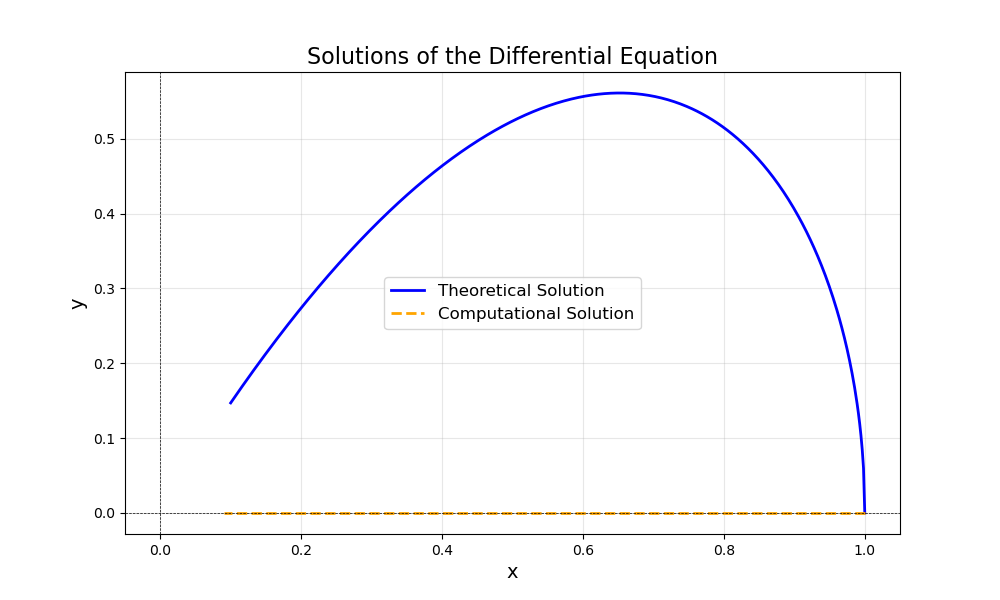
\includegraphics[width = \columnwidth]{figs/Figure_1.png}
	\caption{Solution of given DE}
	\label{fig}
\end{figure}
\end{document}
